\chapter{Osnove logike}

      
             \section{Izjave}

                \textbf{Matematična izjava} je vsaka smiselna poved, za katero 
                lahko določimo resničnost oziroma pravilnost.

                 
                Matematična izjava lahko zavzame dve logični vrednosti:
                \begin{itemize}
                    \item izjava je \textbf{resnična}/\textbf{pravilna}, 
                        oznaka $\mathbf{R}$/$\mathbf{P}$/$\mathbf{1}$/$\mathbf{\top}$;
                    \item izjava je \textbf{neresnična}/\textbf{nepravilna}, 
                        oznaka $\mathbf{N}$/$\mathbf{0}$/$\mathbf{\bot }$.
                \end{itemize}                

                 
                Izjave označujemo z velikimi tiskanimi črkami ($A$, $B$, $C$ ...).
             
         

         
             \begin{naloga}
                Ali so naslednje povedi izjave?
                \begin{itemize}   
                    \item Danes sije sonce.
                    \item Koliko je ura?
                    \item Piramida je geometrijski lik.
                    \item Daj mi jabolko.
                    \item Število $12$ deli število $3$.
                    \item Število $3$ deli število $10$.
                    \item Ali si pisal matematični test odlično?
                    \item Matematični test si pisal odlično.
                    \item Ali je $10~dl$ isto kot $1~l$?
                    \item Število $41$ je praštevilo.
                \end{itemize}
            \end{naloga}
             
         

         
             \begin{naloga}
                Spodnjim izjavam določite logične vrednosti.
                \begin{itemize}   
                    \item $A$: Najvišja gora v Evropi je Mont Blanc.
                    \item $B$: Število je deljivo s $4$ natanko takrat, ko je vsota števk deljiva s $4$.
                    \item $C$: Ostanek pri deljenju s $4$ je lahko $1$, $2$ ali $3$.
                    \item $D$: Mesec februar ima 28 dni.
                    \item $E$: Vsa praštevila so liha števila.
                    \item $F$: Število $1$ je naravno število.
                    \item $G$: Praštevil je neskončno mnogo.
                \end{itemize}
            \end{naloga}
            
         

         
              \subsection{Enostavne in sestavjene izjave}
                
                Izjave delimo med:
                \begin{itemize}
                    \item \textbf{elementarne}/\textbf{enostavne izjave} -- ne moremo 
                        jih razstaviti na bolj enostavne;
                    \item \textbf{sestavljene izjave} -- sestavljene iz elementarnih izjav, 
                        ki jih med seboj povezujejo \textbf{logične operacije} (imenovane 
                        tudi izjavne povezave oziroma~ logična vezja).
                \end{itemize}
             

               
                Vrednost sestavljene izjave izračunamo glede na vrednosti elementarnih 
                izjav in izjavnih povezav med njimi.
             
               
                Pravilnost sestavljenih izjav nazorno prikazujejo 
                \textbf{resničnostne}/\textbf{pravilnostne tabele}.
             

         

         
             \section{Logične operacije}

              \subsection{Negacija}
                \textbf{Negacija} izjave $A$ je izjava, ki \textbf{trdi nasprotno} 
                kot izjava $A$.
                Oznaka: $\mathbf{\lnot A}$.
                $$ \mathbf{\lnot A} \quad \quad \textmd{\textbf{Ni res}, da velja izjava A.}$$
             

                      
                        Če je izjava $A$ pravilna, je $\lnot A$ nepravilna in obratno: 
                        če je $\lnot A$ pravilna, je $A$ nepravilna.
                     
                      
                        Negacija negacije izjave je potrditev izjave. \quad $\lnot(\lnot A)=A$
                     

                \begin{table}[H]
                    \centering
                    \begin{tabular}{||c|c||} 
                    \hhline{|t:==:t|}
                    \rowcolor[rgb]{0.843,0.718,0.718} $A$ & $\lnot A$  \\ 
                    \hhline{|:==:|}
                    $P$                                   & $N$                       \\ 
                    \hline
                    $N$                                   & $P$                       \\
                    \hhline{|b:==:b|}
                    \end{tabular}                    
                \end{table}                

         

         
             \begin{naloga}
                Izjavam določite logično vrednost, potem jih zanikajte in določite logično vrednost negacij.
                \begin{itemize}
                    \item $A$: $5 \cdot 8 = 30$
                    \item $B$: Število $3$ je praštevilo.
                    \item $C$: Največje dvomestno število je $99$.
                    \item $D$: Število $62$ je večratnik števila $4$.
                    \item $E$: Praštevil je neskončno mnogo.
                    \item $F$: $7 \leq 5$
                    \item $G$: Naša pisava je cirilica.
                \end{itemize}
            \end{naloga}
         

         
             \subsection{Konjunkcija}
                \textbf{Konjunkcija} izjav $A$ in $B$ nastane tako, da povežemo izjavi $A$ in $B$ 
                z \textbf{in hkrati}.
                $$ \mathbf{A\land B} \quad \quad \textmd{Velja izjava A \textbf{in (hkrati)} izjava B.}$$
             
                        Če sta izjavi $A$ in $B$ pravilni, je pravilna tudi njuna konjunkcija, 
                        če je pa ena od izjav nepravilna, je nepravilna tudi njuna konjunkcija.
                     

                    \begin{table}[H]
                        \centering
                        \begin{tabular}{||c|c|c||} 
                        \hhline{|t:===:t|}
                        \rowcolor[rgb]{0.843,0.718,0.718} $A$ & $B$ & $A\land B$  \\ 
                        \hhline{|:===:|}
                        $P$ & $P$ & $P$                         \\ 
                        \hline
                        $P$ & $N$ & $N$                         \\ 
                        \hline
                        $N$ & $P$ & $N$                         \\ 
                        \hline
                        $N$ & $N$ & $N$                         \\
                        \hhline{|b:===:b|}
                        \end{tabular}
                    \end{table}



         

         
             \begin{naloga}
                Določite logično vrednost konjunkcijam.
                \begin{itemize}
                    \item Število $28$ je večratnik števila $3$ in večkratnik števila $8$.
                    \item Število $7$ je praštevilo in je deljivo s številom $1$.
                    \item Vsakemu celemu številu lahko pripišemo nasprotno število in obratno celo število.
                    \item Ostanki pri deljenju števila s $3$ so lahko $0$, $1$ ali $2$, 
                        pri deljenju s $5$ pa $0$, $1$, $2$, $3$ ali $4$.
                    \item Število je deljivo s $3$, če je vsota števk deljiva s $3$, in je 
                        deljivo z $9$, če je vsota števk deljiva z $9$.
                \end{itemize}
            \end{naloga}
         

         
             \subsection{Disjunkcija}
                \textbf{Disjunkcija} izjav $A$ in $B$ nastane s povezavo \textbf{ali}.
                $$ \mathbf{A\lor B} \quad \quad \textmd{Velja izjava A \textbf{ali} izjava B 
                (lahko tudi obe hkrati).}$$
             
                      
                        Disjunkcija je nepravilna, če sta nepravilni obe izjavi, ki jo sestavljata,
                        v preostalih treh primerih je pravilna.
                     

                    \begin{table}[H]
                        \centering
                        \begin{tabular}{||c|c|c||} 
                        \hhline{|t:===:t|}
                        \rowcolor[rgb]{0.843,0.718,0.718} $A$ & $B$ & $A\lor B$  \\ 
                        \hhline{|:===:|}
                        $P$ & $P$ & $P$                         \\ 
                        \hline
                        $P$ & $N$ & $P$                         \\ 
                        \hline
                        $N$ & $P$ & $P$                         \\ 
                        \hline
                        $N$ & $N$ & $N$                         \\
                        \hhline{|b:===:b|}
                        \end{tabular}
                    \end{table}



         

         
             \begin{naloga}
                Določite logično vrednost disjunkcijam.
                \begin{itemize}
                    \item Število $24$ je večratnik števila $3$ ali $8$.
                    \item Število $35$ ni večratnik števila $7$ ali $6$.
                    \item Število $5$ deli število $16$ ali $18$.
                    \item Ploščina kvadrata s stranico $a$ je $a^2$ ali obseg kvadrata je $4a$.
                    \item Ni res, da je vsota notranjih kotov trikotnika $160^\circ$, ali ni res, 
                        da Pitagorov izrek velja v poljubnem trikotniku.
                \end{itemize}
            \end{naloga}
         


         
             \subsection{Komutativnost konjunkcije in disjunkcije}
                $$ A\land B = B\land A $$
                $$ A\lor B = B\lor A$$
                   
            
             \subsection{Asociativnost konjunkcije in disjunkcije}
                $$(A\land B)\land C = A\land(B\land C) $$
                $$ (A\lor B)\lor C = A\lor (B\lor C) $$
             

             \subsection{Distributivnost zakona za konjunkcijo in disjunkcijo}
                $$(A\lor B)\land C = (A\land C)\lor(B\land C) $$
                $$ (A\land B)\lor C = (A\lor C)\land(B\lor C) $$
             

             \subsection{De Morganova zakona}
                \begin{itemize}
                    \item negacija konjunkcije je disjunkcija negacij: 
                        $\lnot(A\land B)=\lnot A\lor\lnot B$
                    \item negacija disjunkcije je konjunkcija negacij: 
                        $\lnot(A\lor B)=\lnot A\land\lnot B$
                \end{itemize}                
             
        
         

         
             \begin{naloga}
                Katere od spodnjih izjav so pravilne in katere nepravilne?
                \begin{itemize}
                    \item $(3\cdot 4 = 12)\land(12:4=3)$
                    \item $(a^3\cdot a^5=a^{15})\lor (a^3\cdot a^5=a^8)$
                    \item $(3|30)\land(3|26)$
                    \item $(3|30)\lor(3|26)$
                    \item $(2^3=9)\lor(3^2=9)$
                    \item $((-2)^2=4)\land\lnot(-2^2=4)$
                \end{itemize}
            \end{naloga}
         

         
             \subsection{Implikacija}
                \textbf{Implikacija} izjav $A$ in $B$ je sestavljena izjava, ki jo lahko beremo
                na različne načine.
                $$ \mathbf{A\Rightarrow B} \quad \quad \textmd{\textbf{Če} velja izjava A, 
                \textbf{potem} velja izjava B. / \textbf{Iz} A \textbf{sledi} B.}$$
                Izjava $A$ je \textbf{pogoj} ali \textbf{privzetek}, izjava $B$ pa 
                \textbf{(logična) posledica} izjave $A$.
             
                      
                        Implikacija je nepravilna, ko je izjava $A$ pravilna, izjava $B$ pa 
                        nepravilna, v preostalih treh primerih je pravilna.
                     

                    \begin{table}[H]
                        \centering
                        \begin{tabular}{||c|c|c||} 
                        \hhline{|t:===:t|}
                        \rowcolor[rgb]{0.843,0.718,0.718} $A$ & $B$ & $A\Rightarrow B$  \\ 
                        \hhline{|:===:|}
                        $P$ & $P$ & $P$                         \\ 
                        \hline
                        $P$ & $N$ & $N$                         \\ 
                        \hline
                        $N$ & $P$ & $P$                         \\ 
                        \hline
                        $N$ & $N$ & $P$                         \\
                        \hhline{|b:===:b|}
                        \end{tabular}
                    \end{table}

         

         
             \begin{naloga}
                Določite, ali so izjave pravilne.
                \begin{itemize}
                    \item Če je število deljivo s $100$, je deljivo tudi s $4$.
                    \item Če je štirikotnik pravokotnik, se diagonali razpolavljata.
                    \item Če je štirikotnik kvadrat, se diagonali sekata pod pravim kotom.
                    \item Če sta števili $2$ in $3$ lihi števili, potem je produkt teh dveh števil sodo število.
                    \item Če je število $18$ deljivo z $9$, potem je deljivo s $3$.
                    \item Če je $7$ večkratnik števila $7$, potem $7$ deli število $43$.
                    \item Če je število deljivo s $4$, potem je deljivo z $2$.
                \end{itemize}
            \end{naloga}
         
         
             \subsection{Ekvivalenca}
                \textbf{Ekvivalenca} izjavi $A$ in $B$ poveže s \textbf{če in samo če} oziroma
                \textbf{natanko tedaj, ko}.
                \begin{align*} 
                    \mathbf{A\Leftrightarrow B} \quad \quad &\textmd{Izjava A velja, \textbf{če in
                    samo če} velja izjava B.} / \\
                        &\textmd{Izjava A velja \textbf{natanko tedaj, ko} velja izjava B.}
                \end{align*}
             


                      
                        Ekvivalenca dveh izjav je pravilna, če imata obe izjavi enako vrednost 
                        (ali sta obe pravilni ali obe nepravilni), in nepravilna, če imata izjavi
                        različno vrednost.
                     
                      
                        Ekvivalentni/enakovredni izjavi pomenita eno in isto, lahko ju nadomestimo 
                        drugo z drugo.
                     

                    \begin{table}[H]
                        \centering
                        \begin{tabular}{||c|c|c||} 
                        \hhline{|t:===:t|}
                        \rowcolor[rgb]{0.843,0.718,0.718} $A$ & $B$ & $A\Leftrightarrow B$  \\ 
                        \hhline{|:===:|}
                        $P$ & $P$ & $P$                         \\ 
                        \hline
                        $P$ & $N$ & $N$                         \\ 
                        \hline
                        $N$ & $P$ & $N$                         \\ 
                        \hline
                        $N$ & $N$ & $P$                         \\
                        \hhline{|b:===:b|}
                        \end{tabular}
                    \end{table}


         
             \begin{naloga}
                Določite, ali so naslednje izjave pravilne.
                \begin{itemize}
                    \item Število je deljivo z $12$ natanko takrat, ko je deljivo s $3$ in $4$ hkrati.
                    \item Število je deljivo s $24$ natanko takrat, ko je deljivo s $4$ in $6$ hkrati.
                    \item Število je praštevilo natanko takrat, ko ima natanko dva delitelja.
                    \item Štirikotnik je kvadrat natanko tedaj, ko se diagonali sekata pod pravim kotom.
                    \item Število je sodo natanko tedaj, ko je deljivo z $2$.
                \end{itemize}
            \end{naloga}
         

         
             \subsection{Vrstni red operacij}
                Kadar so izjave povezane z več izjavnimi povezavami, pri določanju logične 
                vrednosti upoštevamo oklepaje in naslednji \textbf{vrstni red} oziroma
                \textbf{prioriteto izjavnih povezav}:
                \begin{enumerate}
                    \item negacija,
                    \item konjunkcija,
                    \item disjunkcija,
                    \item implikacija,
                    \item ekvivalenca.
                \end{enumerate}
             
              
                Če moramo zapored izvesti več enakih izjavnih povezav, velja pravilo združevanja 
                od leve proti desni.
             
         

         
             \begin{naloga}
                V sestavljeni izjavi zapišite oklepaje, ki bodo predstavljali vrstni red operacij.
                Nato tvorite pravilnostno tabelo za sestavljeno izjavo glede na različne logične 
                vrednosti elementarnih izjav.
                \begin{itemize}
                    \item $A\lor B\Leftrightarrow \lnot A\Rightarrow \lnot B$
                    \item $A\lor \lnot A\Rightarrow\lnot B\land (\lnot A\Rightarrow B) $
                    \item $A\Rightarrow B\Leftrightarrow \lnot B\Rightarrow \lnot A $
                    \item $A\land \lnot B\Leftrightarrow A \Rightarrow B$
                    \item $C\Rightarrow A\lor \lnot B\Leftrightarrow \lnot A\land C $
                    \item $\lnot A\lor \lnot B\Leftrightarrow B \land (C\Leftrightarrow \lnot A) $
                \end{itemize}
            \end{naloga}
         

         
             \subsection{Tavtologija in protislovje}

                \textbf{Tavtologija} ali \textbf{logično pravilna izjava} je sestavljena izjava, 
                ki je pri vseh naborih vrednosti elementarnih izjav, iz katerih je sestavjena, pravilna.
             
                \textbf{Protislovje} je sestavljena izjava, ki ni nikoli pravilna.
             

             \subsection{Kvantifikatorja}
                \begin{itemize}
                    \item $\forall$ (beri 'vsak') -- izjava velja za vsak element dane množice
                    \item $\exists$ (beri 'obstaja' ali 'eksistira') -- izjava je pravilna za vsaj en element dane množice
                \end{itemize}
             

         

         
             \section{Pomen izjav v matematiki}
              
                \textbf{Aksiomi} so najpreprostejše izjave, ki so očitno pravilne in zato njihove 
                pravilnosti ni treba dokazovati.
             
              
                \textbf{Izreki} ali \textbf{teoremi} so izjave, ki so pravilne, vendar pa njihova 
                pravilnost ni očitna. 
                Pravilnost izreka (teorema) moramo potrditi z dokazom, ki temelji na aksiomih in na 
                preprostejših že prej dokazanih izrekih.
             
              
                \textbf{Definicije} so izjave, s katerimi uvajamo nove pojme. Najpreprostejših pojmov 
                v matematiki ne opisujemo z definicijami (to so pojmi kot npr.: število, premica ipd.); 
                vsak nadaljnji pojem pa moramo definirati, zato da se nedvoumno ve, o čem govorimo.
             

         
        
\chapter{Osnove teorije množic}


    
        \section{Množice}
        
            \textbf{Množica} je skupek elementov, ki imajo neko skupno lastnost.
        

            Množica je določena, če:
            \begin{itemize}
                \item lahko naštejemo vse njene elemente ali
                \item poznamo pravilo/skupno lastnost, ki pove, kateri elementi so v množici.
            \end{itemize}

            Označujemo jih z velikimi črkami ($\mathcal{A}, \mathcal{B}, \mathcal{C} \dots$ ali  
            $A, B, C \dots$ ). 
            \newline

            \textbf{Univerzalna množica} ali \textbf{univerzum} ($\mathcal{U}$) je množica 
            vseh elementov, ki v danem primeru nastopajo oziroma jih opazujemo.
            \newline
    
            \textbf{Element množice} je objekt v množici. 

            Označujemo jih z malimi črkami ($a, b, c \dots$). 

            Elemente množice zapisujemo v zavitem oklepaju (npr. $\mathcal{A}=\left\{a, b, c\right\}$).

            Element je lahko vsebovan v množici (npr. $a\in\mathcal{A}$) ali pa 
            v množici ni vsebovan (npr. $d\notin\mathcal{A}$).
            \newline

            \textbf{Prazna množica} ($\mathbf{\emptyset, \left\{\right\}}$) je množica, 
            ki ne vsebuje nobenega elementa.
        

    

    
        \section{Moč množice}

            Število elementov v množici predstavlja \textbf{moč množice}.
            Oznaka: $\mathbf{m(\mathcal{A})}$ ali $\mathbf{|\mathcal{A}|}$.
        

            Množica je lahko:
            \begin{itemize}
                \item \textbf{končna množica} -- vsebuje končno mnogo elementov: $\mathbf{m(\mathcal{A})=n}$;
                \item \textbf{neskončna množica} -- vsebuje neskončno mnogo elementov: $\mathbf{m(\mathcal{A})=\infty}$.
            \end{itemize}
        

            Če ima množica toliko elementov, kot jih ima množica naravnih števil, je ta števno 
            neskončna.
            Njeno moč pišemo kot: $m(\mathcal{A})=\aleph_0$.
 
            Za množici, ki imata isto moč, rečemo, da sta \textbf{ekvipolentni} oziroma \textbf{ekvipotentni}.
        

    

    
        \begin{naloga}
            Naštejte elemente množice in zapišite njeno moč, če je $\mathcal{U}=\mathbb{N}$.
            \begin{itemize}
                \item $\mathcal{A}=\{x; x\mid 24\}$
                \item $\mathcal{B}=\{x; 3<x\leq 7\}$
                \item $\mathcal{C}=\{x; x=4k\land k\in\mathbb{N}\land k\leq 5\}$
                \item $\mathcal{D}=\{x; x=3k+2\land k\in\mathbb{N}\land (4<k\leq 8)\}$
            \end{itemize}
        \end{naloga}

        \begin{naloga}
            Naj bo $\mathcal{U}=\mathbb{N}$. Zapišite množico tako, da naštejete njene elemente.
            Določite še njeno moč.
            \begin{itemize}
                \item Množica vseh deliteljev števila 18.
                \item Množica praštevil, ki so manjša od 20.
                \item Množica večkratnikov števila $5$, ki so večji od $50$ in manjši ali enaki $70$.
            \end{itemize}
        \end{naloga}

    

    
        \begin{naloga}
            Zapišite množico s simboli.
            \begin{itemize}
                \item Množica vseh sodih naravnih števil.
                \item Množica vseh naravnih števil, ki dajo pri deljenju s $7$ ostanek $5$.
            \end{itemize}
        \end{naloga}

        \begin{naloga}
            Podane so množice tako, da so našteti njihovi elementi. Množice zapišite s simboli.
            \begin{itemize}
                \item $\mathcal{A}=\{1,2,3,6\}$
                \item $\mathcal{B}=\{6, 12, 18, 24, 30\}$
                \item $\mathcal{C}=\{10, 12, 14, 16, 18, 20\}$
                \item $\mathcal{D}=\{2, 4, 8, 16, 32, 64, 128, 256, 512, 1024\}$
                \item $\mathcal{E}=\{1,4,9,16,25,36,49\}$
            \end{itemize}
        \end{naloga}

    

    \section{Podmnožice}
        
        Množica $\mathcal{B}$ je \textbf{podmnožica} množice $\mathcal{A}$, če za vsak element iz
        $\mathcal{B}$ velja, da je tudi element množice $\mathcal{A}$.
        $$ \mathcal{B}\subseteq\mathcal{A}\Leftrightarrow\forall x\in\mathcal{B}\Rightarrow x\in\mathcal{A} $$
                

        \begin{figure}[H]   
            \centering         
                    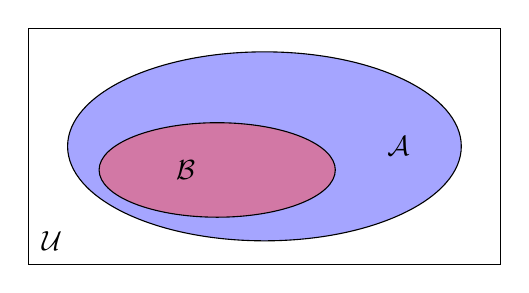
\begin{tikzpicture}                     
                        \draw  (-3,-1.5)  rectangle (3,1.5);
                    
                        \draw[fill=blue!70,fill opacity=0.5] (0,0) ellipse (2.5cm and 1.2cm);
                        \draw[fill=red!70,fill opacity=0.5] (-0.6,-0.3) ellipse (1.5cm and 0.6cm);
                        
                        \node at (-1,-0.3) {$\mathcal{B}$};
                        \node at (1.7,0) {$\mathcal{A}$};
                        % \node at (0,1.1) {$\mathcal{B}\subseteq\mathcal{A}$};
                        \node at (-2.7,-1.2) {$\mathcal{U}$};
                        
                    \end{tikzpicture}
        \end{figure}


          

            \begin{itemize}
                \item $\forall \mathcal{A}:\mathcal{A}\subseteq\mathcal{A}$ -- Vsaka množica je podmnožica
                    same sebe.
                \item $\forall \mathcal{A}:\emptyset\subseteq\mathcal{A}$ -- Prazna množica je podmnožica
                    vsake množice. \newline
            \end{itemize}
            

            Moč podmnožice $\mathcal{B}$ množice $\mathcal{A}$ je manjša ali enaka moči množice $\mathcal{A}$:
            $$\mathcal{B}\subseteq\mathcal{A}\Rightarrow m(\mathcal{B})\leq m(\mathcal{A})$$

    

    
            Množici $\mathcal{A}$ in $\mathcal{B}$ sta \textbf{enaki}, če imata iste elemente; 
            sta druga drugi podmnožici.
            $$\mathcal{A}=\mathcal{B}\Leftrightarrow(\mathcal{A}\subseteq\mathcal{B})\land(\mathcal{B}\subseteq\mathcal{A})$$

            Podmnožica $\mathcal{B}$ množice $\mathcal{A}$, ki ni enaka množici $\mathcal{A}$, 
            je \textbf{prava podmnožica} množice $\mathcal{A}$.
            \newline

            \textbf{Potenčna množica} množice $\mathcal{A}$ je množica vseh podmnožic množice $\mathcal{A}$.
            
            Oznaka: $\mathbf{\mathcal{P}\mathcal{A}}$ / $\mathbf{\mathcal{P}(\mathcal{A})}$.
            $$ \mathcal{PA}=\left\{\mathcal{X}; \mathcal{X}\subseteq\mathcal{A} \right\}$$
        

            $$ m(\mathcal{PA})=2^{m(\mathcal{A})}$$
            Potenčna množica ni nikoli prazna -- vsebuje vsaj prazno množico.
    
    
            \begin{naloga}
                Dana je množica $\mathcal{A}=\{2,4,6,8,10\}$. Zapišite njeno potenčno množico. 
                Kakšna je njena moč?
            \end{naloga}

            \begin{naloga}
                Dana je množica $\mathcal{A}=\{a,b,c,d\}$. Zapiište njeno potenčno množico. 
                Kakšna je njena moč?
            \end{naloga}

        \section{Operacije z množicami}

        \subsection{Komplement množice}
        
                    \textbf{Komplement} množice $\mathcal{A}$ (glede na izbrani univerzum $\mathcal{U}$) je množica 
                    vseh elementov, ki so v množici $\mathcal{U}$ in niso v množici $\mathcal{A}$.

                    Oznaka: $\mathbf{\mathcal{A}^\complement}$ / $\mathbf{\mathcal{A}'}$.      
                    $$ \mathcal{A}^\complement=\left\{ x; x\in\mathcal{U}\land x\notin\mathcal{A}\right\} $$           
                

                \begin{figure}[H]
                    \centering
                    \begin{tikzpicture}                     
                        \draw[fill=red!70,fill opacity=0.5]  (-3,-1.5)  rectangle (3,1.5);
                    
                        % \draw[fill=blue!70,fill opacity=0.5] (0,0) ellipse (2.5cm and 1.2cm);
                        \draw[fill=white,fill opacity=1] (-0.6,-0.3) ellipse (1.5cm and 0.8cm);
                        
                        \node at (-1,-0.3) {$\mathcal{A}$};
                        \node at (1.7,0) {$\mathcal{A}^\complement$};
                        % \node at (0,1.1) {$\mathcal{A}^\complement$};
                        \node at (-2.7,-1.2) {$\mathcal{U}$};
                        
                    \end{tikzpicture}
                \end{figure}

            $$\left( \mathcal{A}^\complement\right)^\complement=\mathcal{A} $$
            
            \begin{naloga}
                Naj bo univerzalna množica $\mathcal{U}=\{x; x\in\mathbb{N} \land x\leq 20\}$. 
                Zapišite komplementarno množico danih množic. Kakšna je njena mmoč?
                \begin{itemize}
                    \item $\mathcal{A}=\{x; x=3k \land k\in\mathbb{N}\}$
                    \item $\mathcal{B}=\{x; x\in\mathbb{N} \land x\mid 20\}$
                    \item $\mathcal{C}=\{x; x=2k \lor x=3k \land k\in\mathbb{N}\}$
                \end{itemize}
            \end{naloga}



        \subsection{Unija množic}
                    \textbf{Unija} množic $\mathcal{A}$ in $\mathcal{B}$ je množica vseh elementov, ki pripadajo 
                    množici $\mathcal{A}$ ali množici $\mathcal{B}$.

                    Oznaka: $\mathbf{\mathcal{A}\cup\mathcal{B}}$.
                    $$ \mathcal{A}\cup\mathcal{B}=\left\{x; x\in\mathcal{A}\lor x\in\mathcal{B}\right\} $$



            \begin{figure}[H]
                \centering
                \begin{subfigure}[b]{0.4\textwidth}
                    \centering
                                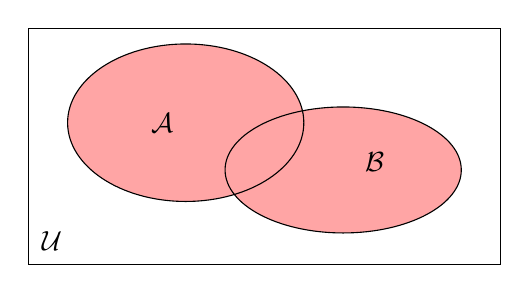
\begin{tikzpicture}                     
                    \draw  (-3,-1.5)  rectangle (3,1.5);
                
                    \draw[fill=red!70,fill opacity=0.5] (-1,0.3) ellipse (1.5cm and 1cm)
                                                        (1,-0.3) ellipse (1.5cm and 0.8cm);
                    
                    \node at (-1.3,0.3) {$\mathcal{A}$};
                    \node at (1.4,-0.2) {$\mathcal{B}$};
                    % \node at (0,1.1) {$\mathcal{A}\cup\mathcal{B}$};
                    \node at (-2.7,-1.2) {$\mathcal{U}$};
                    
                \end{tikzpicture}

                \end{subfigure}
                \begin{subfigure}[b]{0.4\textwidth}
                    \centering
                    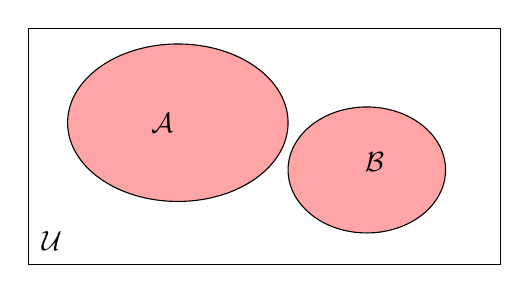
\begin{tikzpicture}                     
                    \draw  (-3,-1.5)  rectangle (3,1.5);
                
                    \draw[fill=red!70,fill opacity=0.5] (-1.1,0.3) ellipse (1.4cm and 1cm)
                                                        (1.3,-0.3) ellipse (1cm and 0.8cm);
                    
                    \node at (-1.3,0.3) {$\mathcal{A}$};
                    \node at (1.4,-0.2) {$\mathcal{B}$};
                    % \node at (0,1.1) {$\mathcal{A}\cup\mathcal{B}$};
                    \node at (-2.7,-1.2) {$\mathcal{U}$};
                    
                \end{tikzpicture}
            \end{subfigure}
        \end{figure}


                    $$ \mathcal{A}\cup\mathcal{A}^\complement=\mathcal{U}$$
                    $$ \mathcal{A}\cup\emptyset=\mathcal{A}$$
                    $$ \mathcal{A}\cup\mathcal{U}=\mathcal{U}$$
                


                    \begin{naloga}
                        Dani sta množici $\mathcal{A}$ in $\mathcal{B}$. Zapišite množico $\mathcal{A}\cup\mathcal{B}$.
                        Določite še njeno moč.
                        \begin{itemize}
                            \item $\mathcal{A}=\{1,2,3,4,5\}$ in $\mathcal{B}=\{3,4,5,6,7\}$
                            \item $\mathcal{A}=\{4,8,12,16,20\}$ in $\mathcal{B}=\{3,6,9,12,15,18\}$
                            \item $\mathcal{A}=\{x; x\in\mathbb{N} \land x\mid 18\}$ in $\mathcal{B}=\{x; x\in\mathbb{N} \land x\mid 21\}$
                            \item $\mathcal{A}=\{5,10,15,20,\dots\}$ in $\mathcal{B}=\{10, 20, 30, 40, 50, \dots\}$
                            \item $\mathcal{A}=\{x; x=6k \land k\in\mathbb{N} \land k\leq 4\}$ in $\mathcal{B}=\{x; x\in\mathbb{N} \land x\mid 12\}$
                        \end{itemize}
                    \end{naloga}
            




    \subsection{Presek množic}
                \textbf{Presek} množic $\mathcal{A}$ in $\mathcal{B}$ je množica vseh elementov, ki hkrati 
                pripadajo množici $\mathcal{A}$ in množici $\mathcal{B}$.

                Oznaka: $\mathbf{\mathcal{A}\cap\mathcal{B}}$.
                $$ \mathcal{A}\cap\mathcal{B}=\left\{x; x\in\mathcal{A}\land x\in\mathcal{B}\right\} $$
            

                \begin{figure}[H]
                    \centering
                    \begin{subfigure}[b]{0.4\textwidth}
                        \centering
                        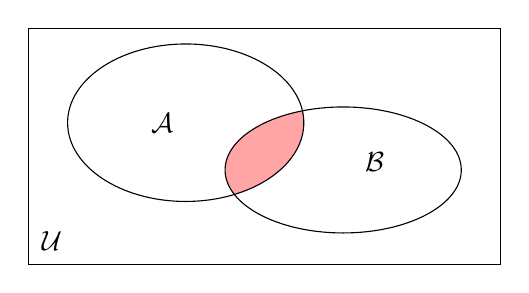
\begin{tikzpicture}                     
                    \draw  (-3,-1.5)  rectangle (3,1.5);

                    \begin{scope}
                        \clip (-1,0.3) ellipse (1.5cm and 1cm);
                        \fill[fill=red!70,fill opacity=0.5] (1,-0.3) ellipse (1.5cm and 0.8cm);
                    \end{scope}
                    \draw (-1,0.3) ellipse (1.5cm and 1cm);
                    \draw (1,-0.3) ellipse (1.5cm and 0.8cm);
                    
                    \node at (-1.3,0.3) {$\mathcal{A}$};
                    \node at (1.4,-0.2) {$\mathcal{B}$};
                    % \node at (0,1.1) {$\mathcal{A}\cap\mathcal{B}$};
                    \node at (-2.7,-1.2) {$\mathcal{U}$};
                    
                \end{tikzpicture}
            \end{subfigure}
            \begin{subfigure}[b]{0.4\textwidth}
                \centering
                    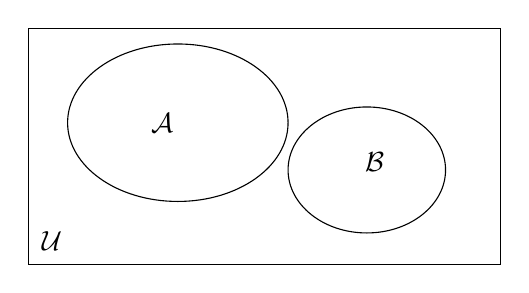
\begin{tikzpicture}                     
                    \draw  (-3,-1.5)  rectangle (3,1.5);
                
                    \draw (-1.1,0.3) ellipse (1.4cm and 1cm)
                        (1.3,-0.3) ellipse (1cm and 0.8cm);
                    
                    \node at (-1.3,0.3) {$\mathcal{A}$};
                    \node at (1.4,-0.2) {$\mathcal{B}$};
                    % \node at (0,1.1) {$\mathcal{A}\cap\mathcal{B}$};
                    \node at (-2.7,-1.2) {$\mathcal{U}$};
                    
                \end{tikzpicture}
            \end{subfigure}
        \end{figure}


                $$ \mathcal{A}\cap\mathcal{A}^\complement=\emptyset$$
                $$ \mathcal{A}\cap\emptyset=\emptyset$$
                $$ \mathcal{A}\cap\mathcal{U}=\mathcal{A}$$



                \begin{naloga}
                    Dani sta množici $\mathcal{A}$ in $\mathcal{B}$. Zapišite množico $\mathcal{A}\cap\mathcal{B}$.
                    Določite še njeno moč.
                    \begin{itemize}
                        \item $\mathcal{A}=\{1,2,3,4,5\}$ in $\mathcal{B}=\{3,4,5,6,7\}$
                        \item $\mathcal{A}=\{4,8,12,16,20\}$ in $\mathcal{B}=\{3,6,9,12,15,18\}$
                        \item $\mathcal{A}=\{x; x\in\mathbb{N} \land x\mid 18\}$ in $\mathcal{B}=\{x; x\in\mathbb{N} \land x\mid 21\}$
                        \item $\mathcal{A}=\{5,10,15,20,\dots\}$ in $\mathcal{B}=\{10, 20, 30, 40, 50, \dots\}$
                        \item $\mathcal{A}=\{x; x=6k \land k\in\mathbb{N} \land k\leq 4\}$ in $\mathcal{B}=\{x; x\in\mathbb{N} \land x\mid 12\}$
                    \end{itemize}
                \end{naloga}
        

    
        Za množici $\mathcal{A}$ in $\mathcal{B}$ velja:
        $$m(\mathcal{A}\cup\mathcal{B})=m(\mathcal{A})+m(\mathcal{B})-m(\mathcal{A}\cap\mathcal{B}) $$
    

    
        Množici, katerih presek je prazna množica, sta \textbf{disjunktni} množici.
        $$\mathcal{A}\cap\mathcal{B}=\emptyset\Rightarrow m(\mathcal{A}\cap\mathcal{B})=0 $$ 
        $$\mathcal{A}\cap\mathcal{B}=\emptyset\Rightarrow m(\mathcal{A}\cup\mathcal{B})=m(\mathcal{A})+m(\mathcal{B}) $$
    

    \subsection{Lastnosti operacij unije in preseka}
            \subsubsection{Komutativnost unije in preseka}
                $$ \mathcal{A}\cup\mathcal{B}=\mathcal{B}\cup\mathcal{A} $$
                $$ \mathcal{A}\cap\mathcal{B}=\mathcal{B}\cap\mathcal{A} $$
            

                \subsubsection{Asociativnost unije in preseka}
                $$ \left(\mathcal{A}\cup\mathcal{B}\right)\cup\mathcal{C}=\mathcal{A}\cup\left(\mathcal{B}\cup\mathcal{C}\right) $$
                $$ \left(\mathcal{A}\cap\mathcal{B}\right)\cap\mathcal{C}=\mathcal{A}\cap\left(\mathcal{B}\cap\mathcal{C}\right) $$


                \subsubsection{Distributivnostna zakona za unijo in presek}
        $$ \left(\mathcal{A}\cup\mathcal{B}\right)\cap\mathcal{C}=\left(\mathcal{A}\cap\mathcal{C}\right)\cup\left(\mathcal{B}\cap\mathcal{C}\right) $$
        $$ \left(\mathcal{A}\cap\mathcal{B}\right)\cup\mathcal{C}=\left(\mathcal{A}\cup\mathcal{C}\right)\cap\left(\mathcal{B}\cup\mathcal{C}\right) $$
    

        \subsubsection{De Morganova zakona}
        Komplement preseka dveh množic je enak uniji komplementov obeh množic:
        $$\left(\mathcal{A}\cap\mathcal{B}\right)^\complement=\mathcal{A}^\complement\cup\mathcal{B}^\complement. $$
        Komplement unije dveh množic je enak preseku komplementov obeh množic:
        $$\left(\mathcal{A}\cup\mathcal{B}\right)^\complement=\mathcal{A}^\complement\cap\mathcal{B}^\complement. $$
    



    
    

            \subsection{Razlika množic}
                \textbf{Razlika} množic $\mathcal{A}$ in $\mathcal{B}$ je množica tistih elementov, ki  
                pripadajo množici $\mathcal{A}$ in hkrati ne pripadajo množici $\mathcal{B}$.

                Oznaka: $\mathbf{\mathcal{A}\setminus\mathcal{B}}$ / $\mathbf{\mathcal{A}-\mathcal{B}}$.
                $$ \mathcal{A}\setminus\mathcal{B}=\left\{x; x\in\mathcal{A}\land x\notin\mathcal{B}\right\} $$
            

            
            


                \begin{figure}[H]
                    \centering
                    \begin{subfigure}[b]{0.4\textwidth}
                        \centering
                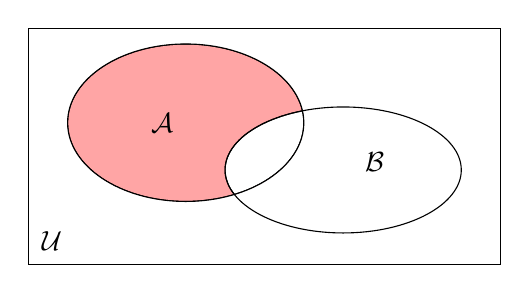
\begin{tikzpicture}                     
                    \draw  (-3,-1.5)  rectangle (3,1.5);

                    \begin{scope}
                        \clip (-1,0.3) ellipse (1.5cm and 1cm);
                        \draw[fill=red!70,fill opacity=0.5, even odd rule] (-1,0.3) ellipse (1.5cm and 1cm)
                                    (1,-0.3) ellipse (1.5cm and 0.8cm);
                    \end{scope}

                    \draw (-1,0.3) ellipse (1.5cm and 1cm);
                    \draw (1,-0.3) ellipse (1.5cm and 0.8cm);
                    
                    \node at (-1.3,0.3) {$\mathcal{A}$};
                    \node at (1.4,-0.2) {$\mathcal{B}$};
                    % \node at (0,1.1) {$\mathcal{A}\setminus\mathcal{B}$};
                    \node at (-2.7,-1.2) {$\mathcal{U}$};
                    
                \end{tikzpicture}
            \end{subfigure}
            \begin{subfigure}[b]{0.4\textwidth}
                \centering
            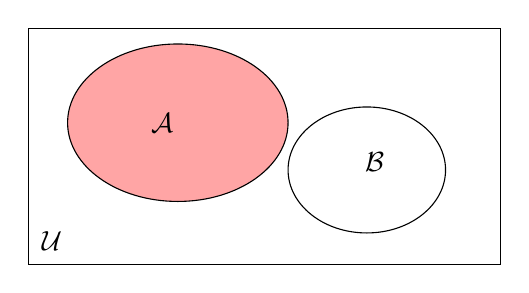
\begin{tikzpicture}                     
                    \draw  (-3,-1.5)  rectangle (3,1.5);
                
                    \draw[fill=red!70,fill opacity=0.5] (-1.1,0.3) ellipse (1.4cm and 1cm);
                    \draw                               (1.3,-0.3) ellipse (1cm and 0.8cm);
                    
                    \node at (-1.3,0.3) {$\mathcal{A}$};
                    \node at (1.4,-0.2) {$\mathcal{B}$};
                    % \node at (0,1.1) {$\mathcal{A}\setminus\mathcal{B}$};
                    \node at (-2.7,-1.2) {$\mathcal{U}$};
                    
                \end{tikzpicture}
            \end{subfigure}
        \end{figure}

    

                $$ \mathcal{A}\setminus\mathcal{B}=\mathcal{A}\cap\mathcal{B}^\complement$$
                $$ \mathcal{A}\setminus\mathcal{B}\neq\mathcal{B}\setminus\mathcal{A}$$
                $$ \mathcal{A}\setminus\mathcal{A}=\emptyset$$


                \begin{naloga}
                    Dani sta množici $\mathcal{A}$ in $\mathcal{B}$. Zapišite njuno razliko $\mathcal{A}\setminus\mathcal{B}$.
                    \begin{itemize}
                        \item $\mathcal{A}=\{2,4,6,8,10,12,14,16,18,20\}$ in $\mathcal{B}=\{x; x\in\mathbb{N} \land x>10\}$
                        \item $\mathcal{A}=\{x; x=3k \land k\in\mathbb{N} \land k<7\}$ in $\mathcal{B}=\{x; x=6k \land k\in\mathbb{N}\}$
                        \item $\mathcal{A}=\{x; x=6k \land k\in\mathbb{N} \land k<4\}$ in $\mathcal{B}=\{x; x=3k \land k\in\mathbb{N}\}$
                    \end{itemize}
                \end{naloga}
    
    

            \subsection{Kartezični produkt množic}
                \textbf{Kartezični produkt} (nepraznih) množic $\mathcal{A}$ in $\mathcal{B}$ je množica 
                urejenih parov $(x,y)$, pri čemer je $x\in\mathcal{A}$ in $y\in\mathcal{B}$.

                Oznaka: $\mathbf{\mathcal{A}\times\mathcal{B}}$.
                $$ \mathcal{A}\times\mathcal{B}=\left\{(x,y); x\in\mathcal{A}\land y\in\mathcal{B}\right\} $$
            

            
                $$x\neq y \Rightarrow (x,y)\neq(y,x)$$
                $$\mathcal{A}\neq\mathcal{B}\Rightarrow \mathcal{A}\times\mathcal{B}\neq\mathcal{B}\times\mathcal{A}$$
            
        
                $$m(\mathcal{A}\times\mathcal{B})=m(\mathcal{A})\cdot m(\mathcal{B}) $$
            \newline

                  Kartezični produkt $\mathcal{A}\times\mathcal{B}$ za množici $ \mathcal{A}=\left\{a,b,c,d,e,f\right\}$ in
                  $ \mathcal{B}=\left\{1,2,3,4\right\}$:

                \begin{figure}[H]  
                    \centering                   
                    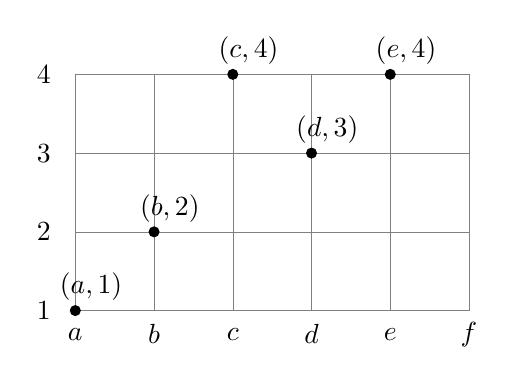
\begin{tikzpicture}
                    \draw[help lines] (0,0) grid (5,3);
                  
                    \fill (1,1) circle (2pt);
                    \fill (3,2) circle (2pt);
                    \fill (2,3) circle (2pt);
                    \fill (4,3) circle (2pt);
                    \fill (0,0) circle (2pt);

                    \node at (0,-0.3) {$a$};
                    \node at (1,-0.3) {$b$};
                    \node at (2,-0.3) {$c$};
                    \node at (3,-0.3) {$d$};
                    \node at (4,-0.3) {$e$};
                    \node at (5,-0.3) {$f$};
                    \node at (-0.4,0) {$1$};
                    \node at (-0.4,1) {$2$};
                    \node at (-0.4,2) {$3$};
                    \node at (-0.4,3) {$4$};

                    \node at (0.2,0.3) {$(a,1)$};
                    \node at (1.2,1.3) {$(b,2)$};
                    \node at (2.2,3.3) {$(c,4)$};
                    \node at (3.2,2.3) {$(d,3)$};
                    \node at (4.2,3.3) {$(e,4)$};

                  \end{tikzpicture}
                \end{figure}

                \begin{naloga}
                    Dani sta množici $\mathcal{A}$ in $\mathcal{B}$. Zapišite njun kartezični produkt $\mathcal{A}\times\mathcal{B}$.
                    Narišite diagram, ki predstavlja to množico.
                    \begin{itemize}
                        \item $\mathcal{A}=\{2,4,6,8,10,12\}$ in $\mathcal{B}=\{x; x\in\mathbb{N} \land x<8\}$
                        \item $\mathcal{A}=\{x; x=3k \land k\in\mathbb{N} \land k < 7\}$ in $\mathcal{B}=\{x; x=6k \land k\in\mathbb{N}\land (5\leq k<9)\}$
                        \item $\mathcal{A}=\{x; x=6k \land k\in\mathbb{N} \land k<4\}$ in $\mathcal{B}=\{x; x=3k \land k\in\mathbb{N}\land (3<k<11)\}$
                    \end{itemize}
                \end{naloga}
        
        
                  


            


    

     
         